\documentclass[alternative-exam.tex]{subfiles}
\begin{document}

\chapter{Matchmaker}
Een matchmaking bureau wil een systeem maken dat hen zegt of een potenti\"ele partner al dan niet goed is voor een bepaalde cli\"ent. Ze ontwikkelen uiteindelijk een systeem dat machine-learning gebruikt om "zijn mening" te geven.

\section{Vraag}
Het bureau vraagt kandidaten een aantal persoonlijke eigenschappen op te geven.
De specifieke mogelijkheden zijn voor elke eigenschap beperkt.
\begin{itemize}
\item Geslacht: man / vrouw
\item Leeftijd: jonger / zelfde / ouder\footnote{De kandidaat moet zijn leeftijd opgeven, maar het systeem houdt enkel bij of de kandidaat jonger of ouder is dan de cli\"ent, of ongeveer dezelfde leeftijd heeft als de cli\"ent.}
\item Muziek: pop / latin / jazz  / klassiek
\item Sport: tennis / golf / joggen / fitness / voetbal
\end{itemize}
De client heeft de vorige kandidaten beoordeeld zoals beschreven in figuur \ref{beoordeling}
\begin{figure}[H]
\centering
\caption{Beoordeling}
\label{beoordeling}
\begin{tabular}{|c|c|c|c|c|}
\hline
geslacht & leeftijd & muziek & sport & beoordeling\\
\hline
vrouw & jonger & latin & joggen & +\\
man & ouder & klassiek & golf & -\\
vrouw & zelfde & pop & tennis & -\\
vrouw & zelfde & klassiek & fitness & +\\
vrouw & jonger & jazz & joggen & +\\
\hline
\end{tabular}
\end{figure}
Aan de hand van de formulering van het systeem heeft het IT departement een hypothesetaal opgesteld zoals beschreven in figuur \ref{hypothesetaal}.
\begin{figure}[H]
\centering
\caption{Hypothesetaal}
\label{hypothesetaal}
\begin{tikzpicture}
\node (s) at (-4,-0.5) {\small Geslacht};
\node (sG) at (-4,-1) {\small ?};
\node (si) at (-5,-2.5) {\small man \tiny m};
\draw[->] (sG) -- (si);
\node (sw) at (-3,-2.5) {\small vrouw \tiny v};
\draw[->] (sG) -- (sw);

%\draw (0,0.5) -- (0,-3);
\node (a) at (4,-0.5) {\small Leeftijd};
\node (aG) at (4,-1) {\small ?};
\node (ay) at (2.5,-2.5) {\small jonger \tiny j};
\draw[->] (aG) -- (ay);
\node (am) at (4,-2.5) {\small zelfde \tiny z};
\draw[->] (aG) -- (am);
\node (ao) at (5.5,-2.5) {\small ouder\tiny o};
\draw[->] (aG) -- (ao);
\end{tikzpicture}\\\vspace{1cm}
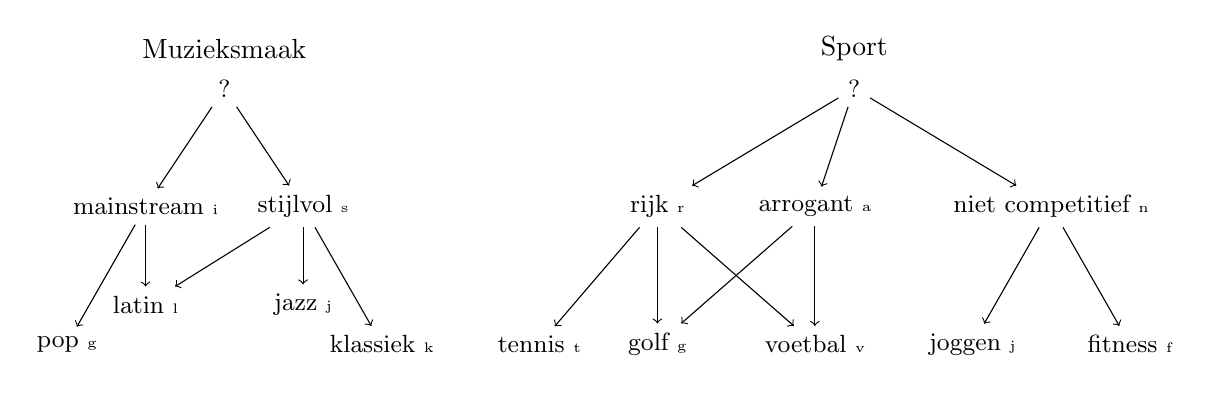
\begin{tikzpicture}
\node (h) at (-4,-0.5) {Muzieksmaak};
\node (hG) at (-4,-1) {\small ?};
\node (hi) at (-5,-2.5) {\small mainstream \tiny i};
\draw[->] (hG) -- (hi);
\node (hig) at (-6,-4.25) {\small pop \tiny g};
\draw[->] (hi) -- (hig);
\node (hil) at (-5,-3.75) {\small latin \tiny l};
\draw[->] (hi) -- (hil);
\node (hr) at (-3,-2.5) {\small stijlvol \tiny s};
\draw[->] (hG) -- (hr);
\draw[->] (hr) -- (hil);
\node (hrs) at (-3,-3.75) {\small jazz \tiny j};
\draw[->] (hr) -- (hrs);
\node (hrf) at (-2,-4.25) {\small klassiek \tiny k};
\draw[->] (hr) -- (hrf);
%\draw (0,0.5) -- (0,-5);
\node (h) at (4,-0.5) {Sport};
\node (hG) at (4,-1) {\small ?};

\node (hi) at (1.5,-2.5) {\small rijk \tiny r};
\draw[->] (hG) -- (hi);
\node (hig) at (0,-4.25) {\small tennis \tiny t};
\draw[->] (hi) -- (hig);
\node (hil) at (1.5,-4.25) {\small golf \tiny g};
\draw[->] (hi) -- (hil);
\node (hv) at (3.5,-2.5) {\small arrogant \tiny a};
\draw[->] (hG) -- (hv);
\node (hiv) at (3.5,-4.25) {\small voetbal \tiny v};
\draw[->] (hv) -- (hiv);
\draw[->] (hi) -- (hiv);
\draw[->] (hv) -- (hil);
\node (hr) at (6.5,-2.5) {\small niet competitief \tiny n};
\draw[->] (hG) -- (hr);
\node (hrs) at (5.5,-4.25) {\small joggen \tiny j};
\draw[->] (hr) -- (hrs);
\node (hrf) at (7.5,-4.25) {\small fitness \tiny f};
\draw[->] (hr) -- (hrf);

\end{tikzpicture}
\end{figure}
Aan het eind van de dag komt er een dame binnen die jonger is dan de client, naar jazz muziek luistert, en elke week gaat joggen. Is deze dame een goede match voor de client, volgens het systeem?

\section{Modeloplossing}
We voeren het version-spaces algoritme uit op de voorbeelden uit de opgave. We beginnen met het initialiseren van $S$ en $G$. $S$ bevat initieel enkel de hypothese die niets aanvaard. $G$ daarentegen, bevat de hypothese die alles aanvaard.
\[
S = \{\bot\}
\]
\[
G = \{[?,?,?,?]\}
\]
\subsection{Iteratie 1}
\begin{figure}
[H]
\centering
\caption{Iteratie 1}
\label{iter_1}
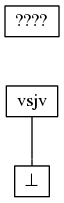
\includegraphics[scale=0.5]{resources/graphs/iteration_1.png}
\end{figure}
Het eerste voorbeeld is een positief voorbeeld. We generaliseren alle hypothesen in $S$ waaraan het voorbeeld niet voldoet. $\bot$ wordt dus gegeneraliseerd naar de hypothese die het voorbeeld precies omvat. Het resultaat zien we in figuur \ref{iter_1}.

\subsection{Iteratie 2}
\begin{figure}
[H]
\centering
\caption{Iteratie 2}
\label{iter_2}
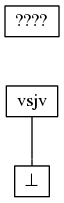
\includegraphics[scale=0.5]{resources/graphs/iteration_2.png}
\end{figure}
Het volgende voorbeeld is negatief beoordeeld. We specifi\"eren alle hypothesen in $G$ waaraan het voorbeeld voldoet. $[m,o,k,g]$ voldoet aan $[?,?,?,?]$ dus we moeten dit specifi\"eren tot het voorbeeld net niet meer aan die nieuwe hypothese(n) voldoet.


\subsection{Iteratie 3}
\begin{figure}
[H]
\centering
\caption{Iteratie 3}
\label{iter_3}
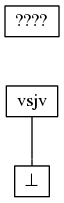
\includegraphics[scale=0.5]{resources/graphs/iteration_3.png}
\end{figure}
\begin{figure}
[H]
\centering
\caption{Iteratie 4}
\label{iter_4}
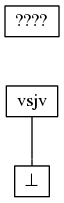
\includegraphics[scale=0.5]{resources/graphs/iteration_4.png}
\end{figure}
\begin{sidewaysfigure}
\centering
\caption{Iteratie 5}
\label{iter_5}
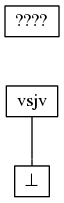
\includegraphics[scale=0.35]{resources/graphs/iteration_5.png}
\end{sidewaysfigure}
\begin{sidewaysfigure}
\centering
\caption{Resultaat}
\label{resultaat}
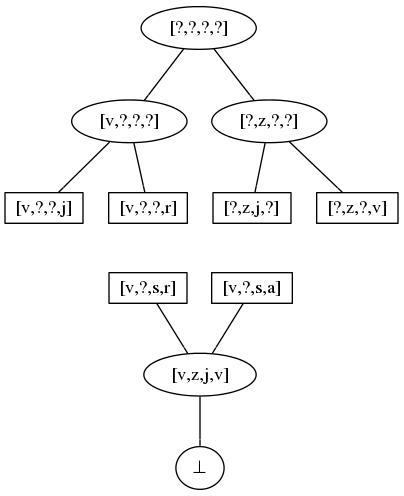
\includegraphics[scale=0.5]{resources/graphs/resultaat.png}
\end{sidewaysfigure}

\end{document}